\documentclass[11pt,a4paper]{article}

% ---- Packages ----
\usepackage[utf8]{inputenc}
\usepackage[T1]{fontenc}
\usepackage{lmodern}
\usepackage[margin=2.5cm]{geometry}
\usepackage{amsmath,amssymb}
\usepackage{graphicx}
\usepackage{booktabs}
\usepackage{array}
\usepackage{float}
\usepackage{caption}
\usepackage{xcolor}
\usepackage{listings}
\usepackage{setspace}
\usepackage[round,authoryear]{natbib}
\usepackage[hidelinks,hypertexnames=false]{hyperref}

\graphicspath{{../figures/}}
\onehalfspacing
\setlength{\parskip}{0.5em}
\setlength{\parindent}{0pt}

% ---- R code style for the appendix ----
\lstdefinestyle{rstyle}{
  language=R,
  basicstyle=\ttfamily\footnotesize,
  keywordstyle=\color{blue!70!black}\bfseries,
  commentstyle=\color{green!45!black}\itshape,
  stringstyle=\color{red!65!black},
  numbers=left,
  numberstyle=\tiny\color{gray},
  stepnumber=1,
  numbersep=6pt,
  breaklines=true,
  breakatwhitespace=false,
  showstringspaces=false,
  frame=single,
  rulecolor=\color{gray!60},
  backgroundcolor=\color{gray!5},
  tabsize=2,
  columns=fullflexible,
  keepspaces=true
}
\lstset{style=rstyle}

\begin{document}

% ---- Title page ----
\begin{titlepage}
  \centering
  \vspace*{3cm}
  {\Large STW7089CEM Introduction to Statistical Methods for Data Science\par}
  \vspace{1cm}
  {\LARGE\bfseries Modelling Cloud Server Power Consumption\\ using Polynomial Regression\par}
  \vspace{0.8cm}
  {\large Coursework (Regular) -- Individual Report\par}
  \vfill
  {\large YOUR NAME\par}
  {\large Student ID: YOUR ID\par}
  \vspace{0.5cm}
  {\large Module Leader: Shrawan Thakur\par}
  \vspace{0.5cm}
  {\large Softwarica College of IT \& E-Commerce\\ in collaboration with Coventry University\par}
  \vspace{0.5cm}
  {\large \today\par}
\end{titlepage}

\pagenumbering{roman}
\tableofcontents
\newpage
\listoffigures
\listoftables
\newpage
\pagenumbering{arabic}

\section*{Abstract}
\addcontentsline{toc}{section}{Abstract}

This report looks for the polynomial regression model that best explains the total power consumption of a simulated cloud server from four telemetry signals: CPU utilisation ($x_1$), memory usage ($x_2$), disk I/O ($x_3$) and network traffic ($x_4$). The dataset has 10{,}000 samples taken every 0.1\,s. Exploratory analysis showed that power is strongly and non-linearly related to disk I/O, weakly related to CPU utilisation, and almost unrelated to memory usage and network traffic when each is looked at on its own. Five candidate models were fitted by least squares and compared using the residual sum of squares, the Gaussian log-likelihood, AIC, BIC and the shape of the residual distribution. Model~2, $y=\theta_1x_4+\theta_2x_1^3+\theta_3x_3^4+\theta_{bias}$, had the lowest AIC and BIC and normally distributed residuals. On a 30\% hold-out test set it reached an RMSE of 5.04\,W and $R^2=0.99996$. Rejection ABC on its two largest parameters gave narrow posteriors centred on the least squares values, with a clear negative correlation between the intercept and the network coefficient.


% ---- Main sections ----
\section{Introduction}

Data centres use a large and growing share of the world's electricity, and most of this energy is drawn by the servers themselves. Knowing how much power a server draws under a given workload helps operators plan power provisioning, place virtual machines on hosts, and spot hardware that behaves abnormally \citep{fan2007}. Power can be measured directly with hardware meters, but these are expensive and hard to deploy on every machine. A cheaper option is to predict power from software telemetry, such as CPU, memory, disk and network load, which every operating system already reports. This only works if the mathematical link between the load signals and the power draw is known. Real servers are also not \emph{energy proportional}: they use a large share of their peak power even when idle, and power grows non-linearly with load \citep{barroso2007}. A simple straight-line model is therefore unlikely to be enough.

The coursework provides simulated telemetry for one server in three files:
\begin{itemize}
  \item \texttt{X.csv}: four input signals, $x_1$ (CPU utilisation), $x_2$ (memory usage), $x_3$ (disk I/O) and $x_4$ (network traffic);
  \item \texttt{y.csv}: the output signal $y$, the total power consumption;
  \item \texttt{time.csv}: the sampling time of each row, in seconds.
\end{itemize}
All five signals contain additive, independent, zero-mean Gaussian noise of unknown variance.

The aim is to find which of five given polynomial models ``truly'' describes the relationship between the inputs and $y$. The report follows the three coursework tasks:
\begin{enumerate}
  \item \textbf{Task 1} -- exploratory analysis of the signals: time series, distributions, correlations and scatter plots (Section~\ref{sec:task1}).
  \item \textbf{Task 2} -- least squares fitting of the five candidate models, model comparison with RSS, log-likelihood, AIC, BIC and residual analysis, and validation of the chosen model on a train/test split (Section~\ref{sec:task2}).
  \item \textbf{Task 3} -- rejection Approximate Bayesian Computation (ABC) to estimate the posterior distribution of the two largest parameters of the chosen model (Section~\ref{sec:task3}).
\end{enumerate}
Section~\ref{sec:discussion} discusses the results and their limits, and Section~\ref{sec:conclusion} concludes. All analysis was done in R version 4.6.1 \citep{rcore2026} using only base R functions. The full annotated code is in Appendix~\ref{app:code}, and the code that produced each result is referenced in the text.

\section{Data and Methodology}
\label{sec:method}

\subsection{Data preparation}
The three CSV files were read into R and joined column by column into one data frame with the columns \texttt{time}, \texttt{x1}, \texttt{x2}, \texttt{x3}, \texttt{x4} and \texttt{y} (Appendix~\ref{app:task1}). There are $n=10{,}000$ rows, sampled every 0.1\,s from 0 to 999.9\,s. No value was missing, so no rows were removed or imputed.

\subsection{Candidate models}
The five candidate models given in the brief are:
\begin{align*}
\text{Model 1:}\quad & y=\theta_1x_4+\theta_2x_1^2+\theta_3x_1^3+\theta_4x_2^4+\theta_5x_1^4+\theta_{bias}+\varepsilon\\
\text{Model 2:}\quad & y=\theta_1x_4+\theta_2x_1^3+\theta_3x_3^4+\theta_{bias}+\varepsilon\\
\text{Model 3:}\quad & y=\theta_1x_3^3+\theta_2x_3^4+\theta_{bias}+\varepsilon\\
\text{Model 4:}\quad & y=\theta_1x_2+\theta_2x_1^3+\theta_4x_3^4+\theta_{bias}+\varepsilon\\
\text{Model 5:}\quad & y=\theta_1x_4+\theta_2x_1^2+\theta_3x_1^3+\theta_4x_3^4+\theta_{bias}+\varepsilon
\end{align*}
The brief numbers the parameters of Model~4 as $\theta_1,\theta_2,\theta_4$ with no $\theta_3$. This looks like a typing error, so Model~4 is treated as having three regressors plus a bias, that is $k=4$ parameters.

Each model is non-linear in the inputs but \emph{linear in the parameters}. Each can therefore be written as $\mathbf{y}=\mathbf{X}\boldsymbol{\theta}+\boldsymbol{\varepsilon}$, where each column of the design matrix $\mathbf{X}$ is one transformed input (for example $x_1^3$) and the last column is all ones for the bias.

\subsection{Statistical methods}
\textbf{Least squares.} The parameters are estimated by ordinary least squares,
\begin{equation}
\hat{\boldsymbol{\theta}}=(\mathbf{X}^T\mathbf{X})^{-1}\mathbf{X}^T\mathbf{y},
\label{eq:ls}
\end{equation}
which is also the maximum likelihood estimate when the noise is i.i.d.\ Gaussian \citep{montgomery2012}.

\textbf{Goodness of fit.} The residual sum of squares is $\text{RSS}=\sum_{i=1}^{n}(y_i-\mathbf{x}_i\hat{\boldsymbol{\theta}})^2$. With the noise variance estimated as $\hat\sigma^2=\text{RSS}/(n-1)$, as the brief specifies, the Gaussian log-likelihood is
\begin{equation}
\ln p(D\mid\hat{\boldsymbol{\theta}})=-\frac{n}{2}\ln(2\pi)-\frac{n}{2}\ln(\hat\sigma^2)-\frac{1}{2\hat\sigma^2}\text{RSS}.
\label{eq:loglik}
\end{equation}

\textbf{Information criteria.} Adding parameters always lowers the RSS, so models of different sizes are compared with
\begin{equation}
\text{AIC}=2k-2\ln p(D\mid\hat{\boldsymbol{\theta}}),\qquad
\text{BIC}=k\ln(n)-2\ln p(D\mid\hat{\boldsymbol{\theta}}),
\label{eq:aicbic}
\end{equation}
where $k$ is the number of estimated parameters \citep{akaike1974,schwarz1978}. Lower values are better. BIC penalises each extra parameter by $\ln(10000)\approx9.2$ instead of 2, so it favours smaller models more strongly than AIC.

\textbf{Residual checks.} If a model has the right structure, its residuals should look like the Gaussian noise in the data. This was checked with histograms, normal Q-Q plots and the Shapiro--Wilk test \citep{shapiro1965}.

\textbf{Validation and intervals.} The chosen model was refitted on a random 70\% of the data and tested on the other 30\%. For a test input $\mathbf{x}_*$, the 95\% confidence interval of the mean prediction is $\hat y_*\pm t_{0.975,\,n_{tr}-k}\sqrt{\mathbf{x}_*^T\hat{\boldsymbol\Sigma}_\theta\mathbf{x}_*}$, with $\hat{\boldsymbol\Sigma}_\theta=\hat\sigma^2(\mathbf{X}^T\mathbf{X})^{-1}$. The 95\% prediction interval for a new observation adds the noise variance $\hat\sigma^2$ inside the square root \citep{james2013}.

\textbf{Rejection ABC.} Parameter values are drawn from a prior. Each draw is used to generate model output, and a draw is kept only if that output is close enough to the observed data. The kept draws approximate the posterior distribution \citep{pritchard1999,beaumont2002,sunnaker2013}. Section~\ref{sec:task3} gives the details.

\section{Task 1: Preliminary Data Analysis}
\label{sec:task1}

Before fitting any model, the five signals were explored to understand their range, shape and dependencies. Table~\ref{tab:summary} gives the summary statistics, produced by the \texttt{summary()}, \texttt{sd()} and skewness lines of the Task~1 script (Appendix~\ref{app:task1}).

\begin{table}[H]
\centering
\caption{Summary statistics of the five signals ($n=10{,}000$).}
\label{tab:summary}
\begin{tabular}{lrrrrrrr}
\toprule
Signal & Min & Q1 & Median & Mean & Q3 & Max & Skewness \\
\midrule
$x_1$ CPU      & 1.00  & 2.72  & 4.45  & 4.46  & 6.18  & 8.00  & 0.03 \\
$x_2$ Memory   & 2.00  & 3.78  & 5.54  & 5.53  & 7.30  & 9.00  & $-0.02$ \\
$x_3$ Disk I/O & $-0.78$ & 3.99 & 5.01 & 5.00 & 6.01 & 11.72 & 0.01 \\
$x_4$ Network  & 0.00  & 0.87  & 2.08  & 3.00  & 4.14  & 27.36 & 1.94 \\
$y$ Power      & 121.7 & 507.1 & 828.3 & 1084.1 & 1375.9 & 15241.3 & 2.71 \\
\bottomrule
\end{tabular}
\end{table}

\subsection{Task 1.1: Time series plots}
Figure~\ref{fig:ts} plots every signal against time over the full 1000\,s. With 10{,}000 points the plots turn into dense bands. They still show that no signal has a trend, a level shift or a change in spread over time: all five are stationary. Disk I/O ($x_3$) varies around a level of about 5. Network traffic ($x_4$) sits near zero with frequent short spikes. Power ($y$) shows the same spiky shape, with a few very large peaks of up to about 15{,}000\,W.

\begin{figure}[H]
\centering
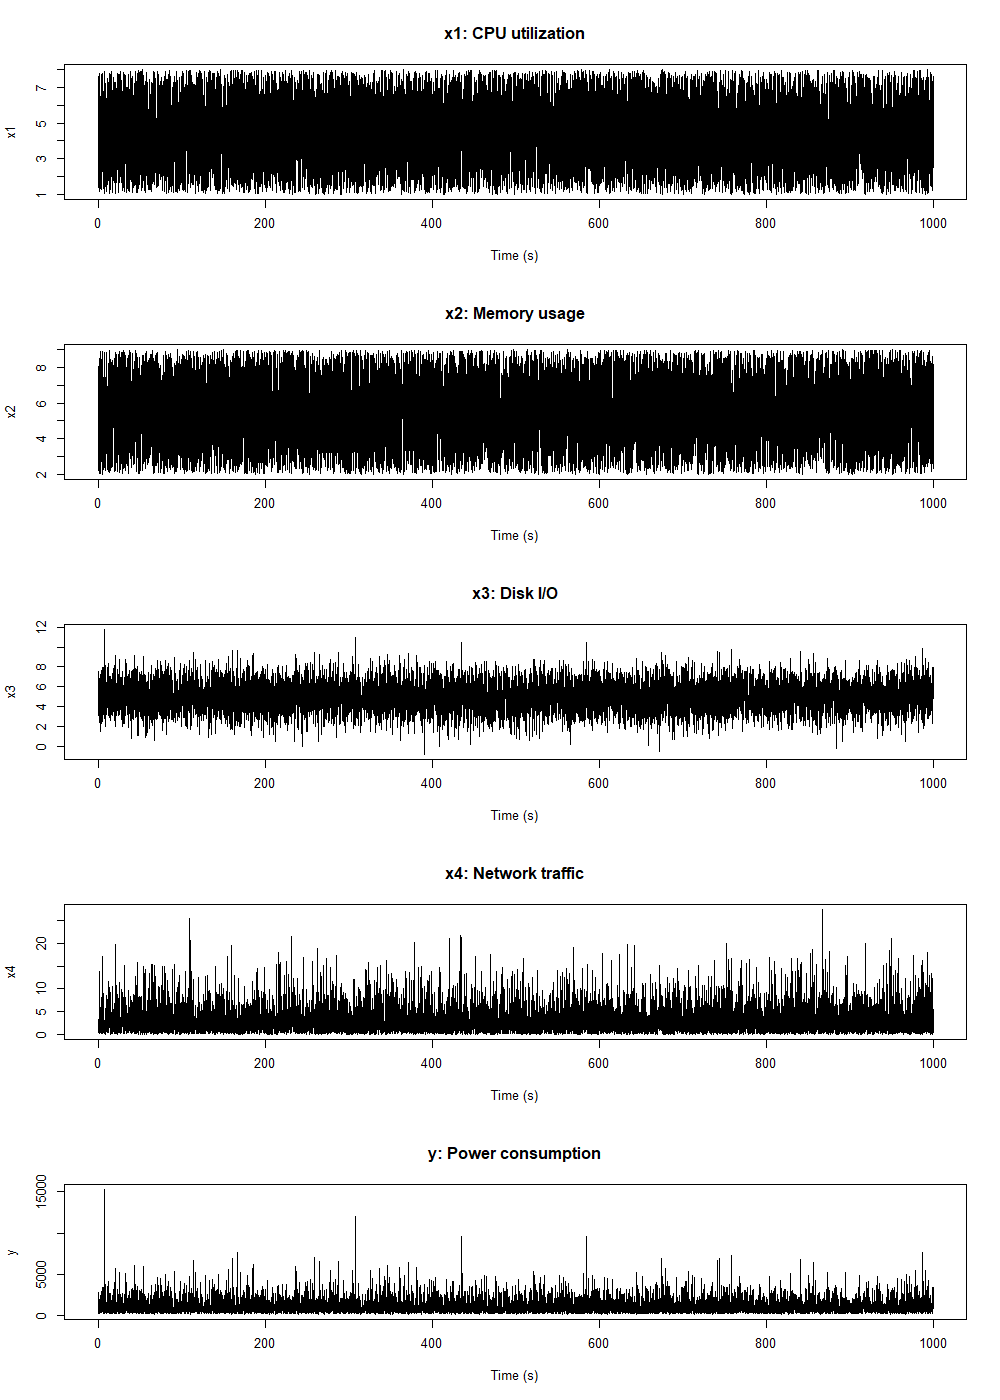
\includegraphics[width=0.78\textwidth]{fig1_time_series.png}
\caption{Time series of the four inputs and the output power over the full 1000\,s record.}
\label{fig:ts}
\end{figure}

Figure~\ref{fig:tszoom} zooms in on the first 20\,s (200 samples) so that single samples can be seen. Neighbouring samples are not similar: each value looks like a fresh random draw, with no cycles or smooth movements. The lag-1 autocorrelation of every signal is between $-0.012$ and $0.011$, which confirms this. The samples can therefore be treated as independent observations, which the regression assumption of i.i.d.\ errors needs. The time stamp carries no useful information for modelling. The plot also shows that the large power spike at about 7\,s happens at the same time as a spike in disk I/O, which is a first hint that $y$ depends strongly on $x_3$.

\begin{figure}[H]
\centering
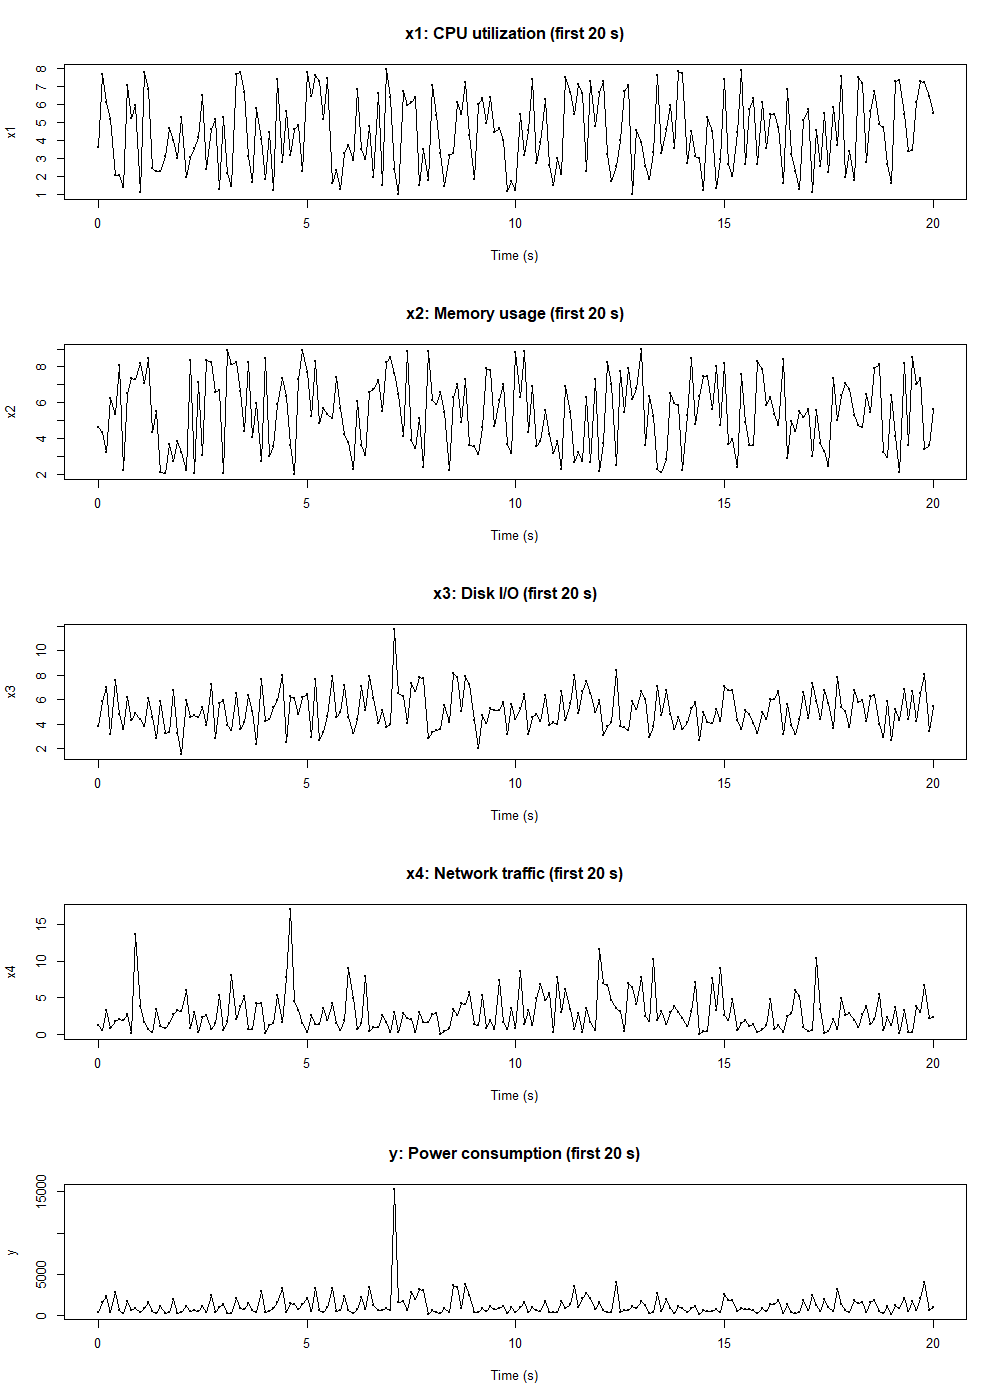
\includegraphics[width=0.78\textwidth]{fig1b_time_series_zoom.png}
\caption{Zoomed time series of the first 20\,s (200 samples).}
\label{fig:tszoom}
\end{figure}

\subsection{Task 1.2: Distribution of each signal}
Figure~\ref{fig:dist} shows a histogram of each signal with a kernel density curve. The four inputs have clearly different shapes:
\begin{itemize}
  \item $x_1$ (CPU) and $x_2$ (memory) are flat between about 1--8 and 2--9. They look \textbf{uniformly distributed}, and the dips at the edges of the density curve are only a smoothing effect.
  \item $x_3$ (disk I/O) is bell-shaped and symmetric around 5 (skewness 0.01). It looks \textbf{normally distributed}, with standard deviation about 1.5.
  \item $x_4$ (network) is strongly \textbf{right-skewed} (skewness 1.94). Its mean (3.0) equals its standard deviation (3.0) and it never goes below zero, which matches an exponential distribution.
  \item $y$ (power) is also strongly right-skewed (skewness 2.71) with a long upper tail.
\end{itemize}
The output is skewed even though $x_3$ is symmetric, which suggests that $y$ depends on a high power of an input: raising a symmetric variable to the fourth power stretches its upper tail.

\begin{figure}[H]
\centering
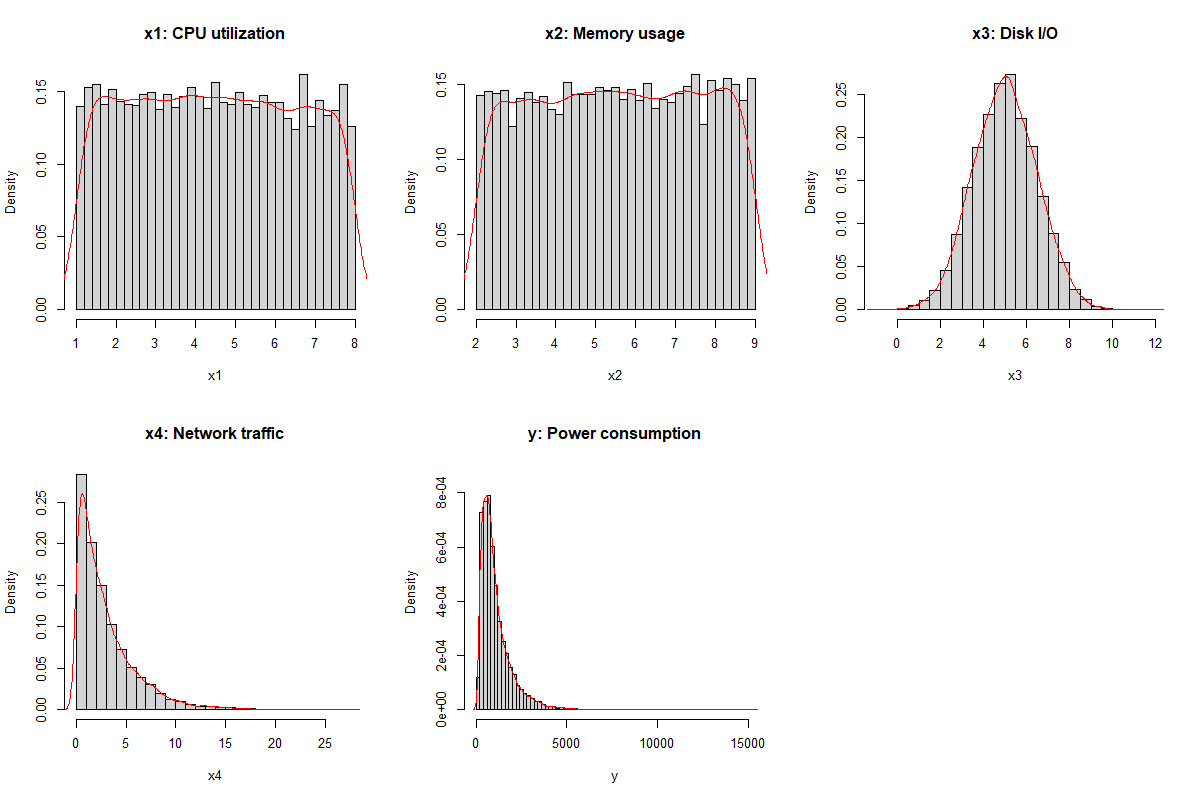
\includegraphics[width=0.95\textwidth]{fig2_distributions.png}
\caption{Histograms with kernel density estimates (red) for each signal.}
\label{fig:dist}
\end{figure}

\subsection{Task 1.3: Correlation and scatter plots}
Table~\ref{tab:cor} and Figure~\ref{fig:corr} give the correlation between all pairs of signals. The inputs are almost uncorrelated with each other ($|r|\le0.023$), so there is no multicollinearity and the effect of each input can be estimated separately. Against the output:
\begin{itemize}
  \item $x_3$ has a strong positive correlation ($r=0.851$). Its Spearman rank correlation is even higher (0.931), which shows that the relationship is monotonic but \emph{not} linear.
  \item $x_1$ has a weak positive correlation ($r=0.174$, Spearman 0.291).
  \item $x_2$ ($r=-0.014$) and $x_4$ ($r=0.010$) show no visible correlation.
\end{itemize}

\begin{table}[H]
\centering
\caption{Correlation of each input with the output $y$.}
\label{tab:cor}
\begin{tabular}{lcccc}
\toprule
 & $x_1$ & $x_2$ & $x_3$ & $x_4$ \\
\midrule
Pearson $r$ with $y$   & 0.174 & $-0.014$ & 0.851 & 0.010 \\
Spearman $\rho$ with $y$ & 0.291 & $-0.012$ & 0.931 & 0.016 \\
\bottomrule
\end{tabular}
\end{table}

\begin{figure}[H]
\centering
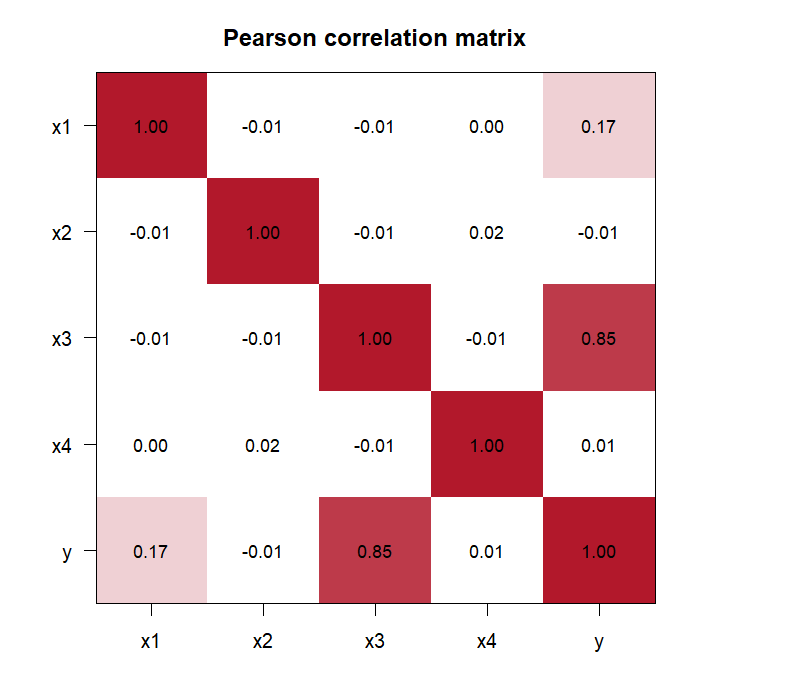
\includegraphics[width=0.6\textwidth]{fig3a_correlation.png}
\caption{Pearson correlation matrix of all signals.}
\label{fig:corr}
\end{figure}

The scatter plots in Figure~\ref{fig:scatter} show the shape of each relationship. The plot of $y$ against $x_3$ shows a clear, tight, upward curve that gets steeper as $x_3$ grows, which is typical of a high-order polynomial term. The plot against $x_1$ shows a lower boundary of the point cloud that rises with $x_1$, so $x_1$ has a smaller non-linear effect that is hidden by the spread caused by $x_3$. The plots against $x_2$ and $x_4$ have flat LOWESS lines.

A low correlation does not prove that an input has no effect. The spread in $y$ caused by $x_3$ (standard deviation 884\,W) is so large that a small linear effect of $x_4$ cannot be seen in a two-variable plot. This is why the models must be compared with all inputs together, as in Task~2.

\begin{figure}[H]
\centering
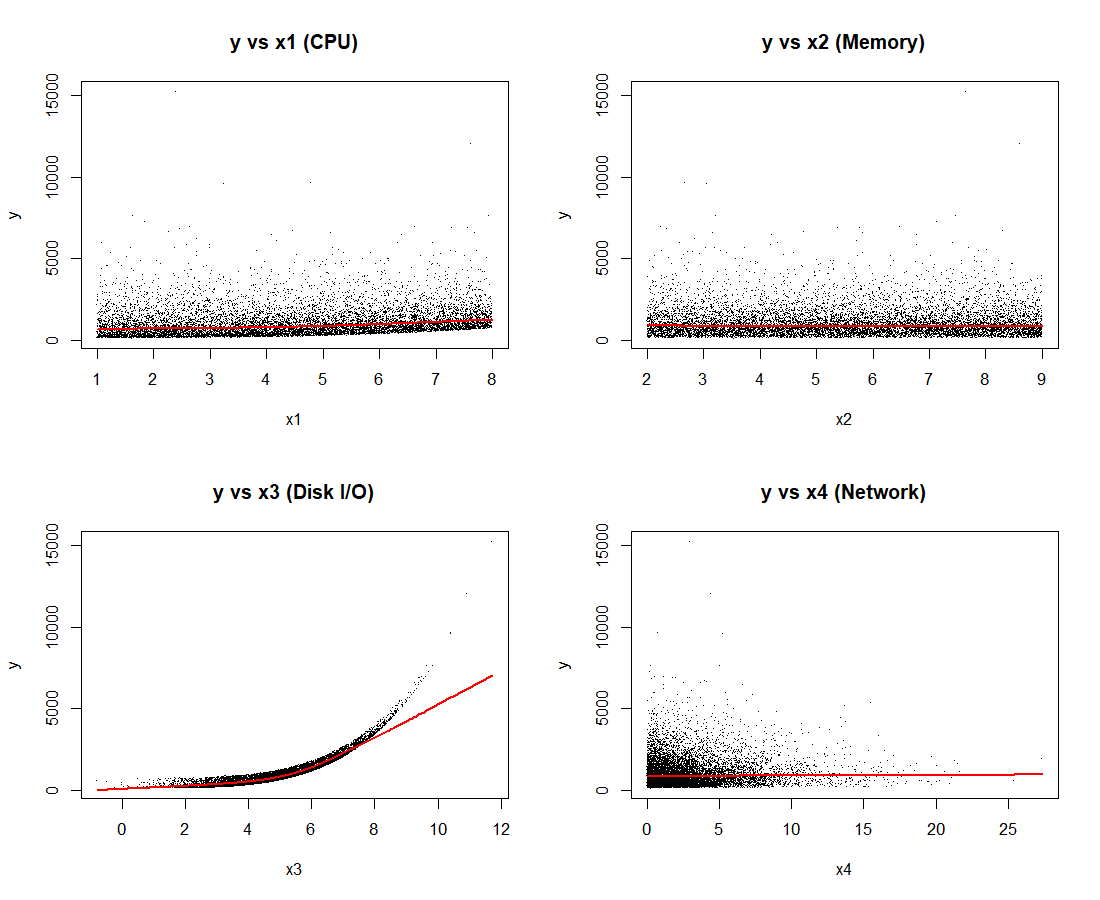
\includegraphics[width=0.85\textwidth]{fig3_scatter.png}
\caption{Scatter plots of the output power against each input, with LOWESS curves (red).}
\label{fig:scatter}
\end{figure}

\subsection{Baseline linear model}
As a reference, a linear model with all four inputs was fitted with \texttt{lm()}. It explains 75.9\% of the variance ($R^2=0.7587$) with a residual standard error of 434.1\,W. $x_1$, $x_3$ and $x_4$ are significant ($p<0.001$), but $x_2$ is not ($p=0.46$). The residual plots in Figure~\ref{fig:linres} show that the linear model is not adequate. The residuals form a curved pattern against the fitted values, and the Q-Q plot bends sharply upwards in the right tail. Both signs mean that the true relationship is non-linear, which supports using the polynomial models of Task~2.

\begin{figure}[H]
\centering
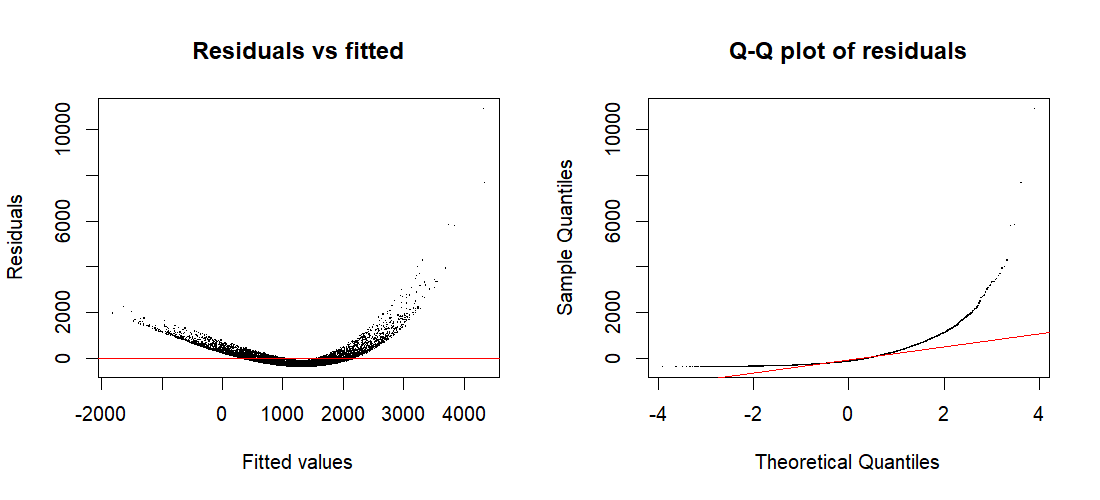
\includegraphics[width=0.85\textwidth]{fig4_linear_residuals.png}
\caption{Residuals vs fitted values and normal Q-Q plot for the baseline linear model.}
\label{fig:linres}
\end{figure}

\section{Task 2: Regression -- Modelling the Relationship between Server Metrics}
\label{sec:task2}

\subsection{Task 2.1: Least squares parameter estimates}
For each model a design matrix was built from the transformed inputs plus a column of ones, and Equation~\eqref{eq:ls} was solved with \texttt{solve(t(X) \%*\% X) \%*\% t(X) \%*\% y} using all 10{,}000 samples (Appendix~\ref{app:task2}, section ``Task 2.1''). As a check, Model~1 was also fitted with \texttt{lm()}, which gave the same estimates to every printed digit. Table~\ref{tab:theta} lists the results.

\begin{table}[H]
\centering
\caption{Least squares estimates $\hat{\boldsymbol\theta}$ for the five candidate models (all data).}
\label{tab:theta}
\begin{tabular}{lll}
\toprule
Model & Term & Estimate \\
\midrule
1 & $x_4$ / $x_1^2$ / $x_1^3$ & 3.0940 / $-4.0550$ / 2.3840 \\
  & $x_2^4$ / $x_1^4$ / bias & $-0.005608$ / $-0.09913$ / 930.83 \\
\midrule
2 & $x_4$ / $x_1^3$ / $x_3^4$ & 4.4805 / 1.20018 / 0.800003 \\
  & bias & 120.022 \\
\midrule
3 & $x_3^3$ / $x_3^4$ / bias & $-0.03076$ / 0.80153 / 308.585 \\
\midrule
4 & $x_2$ / $x_1^3$ / $x_3^4$ & 0.1170 / 1.20032 / 0.79994 \\
  & bias & 132.854 \\
\midrule
5 & $x_4$ / $x_1^2$ / $x_1^3$ & 4.4805 / $-0.01019$ / 1.20146 \\
  & $x_3^4$ / bias & 0.800003 / 120.083 \\
\bottomrule
\end{tabular}
\end{table}

The estimates already show a pattern. Every model that contains $x_3^4$ estimates its coefficient as about 0.80, and every model that contains $x_1^3$ estimates about 1.20. Models~2 and~5 give almost the same values for every shared term ($x_4\approx4.48$, bias $\approx120$), and the extra $x_1^2$ term in Model~5 is close to zero ($-0.010$). Model~1 has no $x_3$ term at all, so its intercept (930.8) is pulled towards the mean of $y$ to make up for it.

\subsection{Task 2.2: Residual sum of squares}
The RSS of each model (Appendix~\ref{app:task2}, ``Task 2.2'') is given in Table~\ref{tab:crit}. The RSS values differ by more than four orders of magnitude. Models~2 and~5 have by far the lowest RSS (about $2.51\times10^5$). The models without the right terms are much worse: Model~4 swaps $x_4$ for $x_2$ ($2.06\times10^6$), Model~3 has no CPU or network term ($3.05\times10^8$), and Model~1 has no disk term ($7.54\times10^9$). This agrees with Task~1, where $x_3$ was found to be the main driver of power.

\subsection{Task 2.3: Log-likelihood}
The variance $\hat\sigma^2=\text{RSS}/(n-1)$ and the log-likelihood from Equation~\eqref{eq:loglik} were computed for each model. For Models~2 and~5, $\hat\sigma^2\approx25.08$, so the noise standard deviation is about 5.0\,W. This is very small next to the spread of $y$ (884\,W), and suggests that these models capture almost all of the signal. Because $\hat\sigma^2$ is proportional to the RSS, the log-likelihood ranks the models in the same order as the RSS.

\subsection{Task 2.4: AIC and BIC}
AIC and BIC were computed from Equation~\eqref{eq:aicbic} with $k$ equal to the number of columns of each design matrix, including the bias. Table~\ref{tab:crit} collects all the criteria. $\Delta$AIC and $\Delta$BIC show the difference from the best model.

\begin{table}[H]
\centering
\caption{Model comparison criteria ($n=10{,}000$). The lowest AIC and BIC (selected model) are in bold.}
\label{tab:crit}
\small
\setlength{\tabcolsep}{4pt}
\begin{tabular}{crrrrrrrr}
\toprule
Model & $k$ & RSS & $\hat\sigma^2$ & $\ln p(D|\hat\theta)$ & AIC & BIC & $\Delta$AIC & $\Delta$BIC \\
\midrule
1 & 6 & $7.538\times10^{9}$ & 753871.8 & $-81853.8$ & 163719.6 & 163762.8 & 103111.7 & 103126.1 \\
2 & 4 & $2.508\times10^{5}$ & 25.08 & $-30300.0$ & \textbf{60607.9} & \textbf{60636.7} & \textbf{0.0} & \textbf{0.0} \\
3 & 3 & $3.048\times10^{8}$ & 30478.8 & $-65812.8$ & 131631.7 & 131653.3 & 71023.8 & 71016.5 \\
4 & 4 & $2.056\times10^{6}$ & 205.65 & $-40819.7$ & 81647.5 & 81676.3 & 21039.6 & 21039.6 \\
5 & 5 & $2.508\times10^{5}$ & 25.08 & $-30299.8$ & 60609.6 & 60645.6 & 1.7 & 8.9 \\
\bottomrule
\end{tabular}
\end{table}

Model~2 has the lowest AIC (60607.9) and the lowest BIC (60636.7). Model~5 comes a close second. Its RSS is only 8.3 lower than that of Model~2 ($250802.2$ against $250810.5$), which raises its log-likelihood by just 0.17. That is far too little to pay for the extra parameter, so its AIC is 1.67 higher and its BIC 8.88 higher. Models~1, 3 and~4 are worse by tens of thousands of units and can be ruled out.

\subsection{Task 2.5: Distribution of the residuals}
Figure~\ref{fig:res} shows a histogram and a normal Q-Q plot of the residuals of each model (Appendix~\ref{app:task2}, ``Task 2.5''). Since the noise in the data is Gaussian, the correct model should leave residuals that are Gaussian too.
\begin{itemize}
  \item \textbf{Model 1}: the residuals are very right-skewed and range up to about 14{,}000. The Q-Q plot curves sharply upwards. The missing $x_3^4$ effect remains in the errors.
  \item \textbf{Model 3}: the residuals are bimodal and spread from $-200$ to 500, and the Q-Q plot has an S-shape. Leaving out $x_1^3$ creates this large structured error, because CPU utilisation is uniform and adds a flat-topped component.
  \item \textbf{Model 4}: the residuals are right-skewed with a long upper tail of up to about 100, because $x_2$ cannot stand in for the skewed network signal $x_4$.
  \item \textbf{Models 2 and 5}: the histograms are symmetric and bell-shaped, centred on zero and within about $\pm18$. The Q-Q points lie on the reference line along the whole range. The two plots cannot be told apart.
\end{itemize}

The Shapiro--Wilk test, applied to the same random 5000 residuals for each model (the R function accepts at most 5000), agrees. Normality is not rejected for Model~2 ($p=0.696$) or Model~5 ($p=0.689$), but is strongly rejected for Models~1, 3 and~4 (all $p<10^{-50}$).

\begin{figure}[H]
\centering
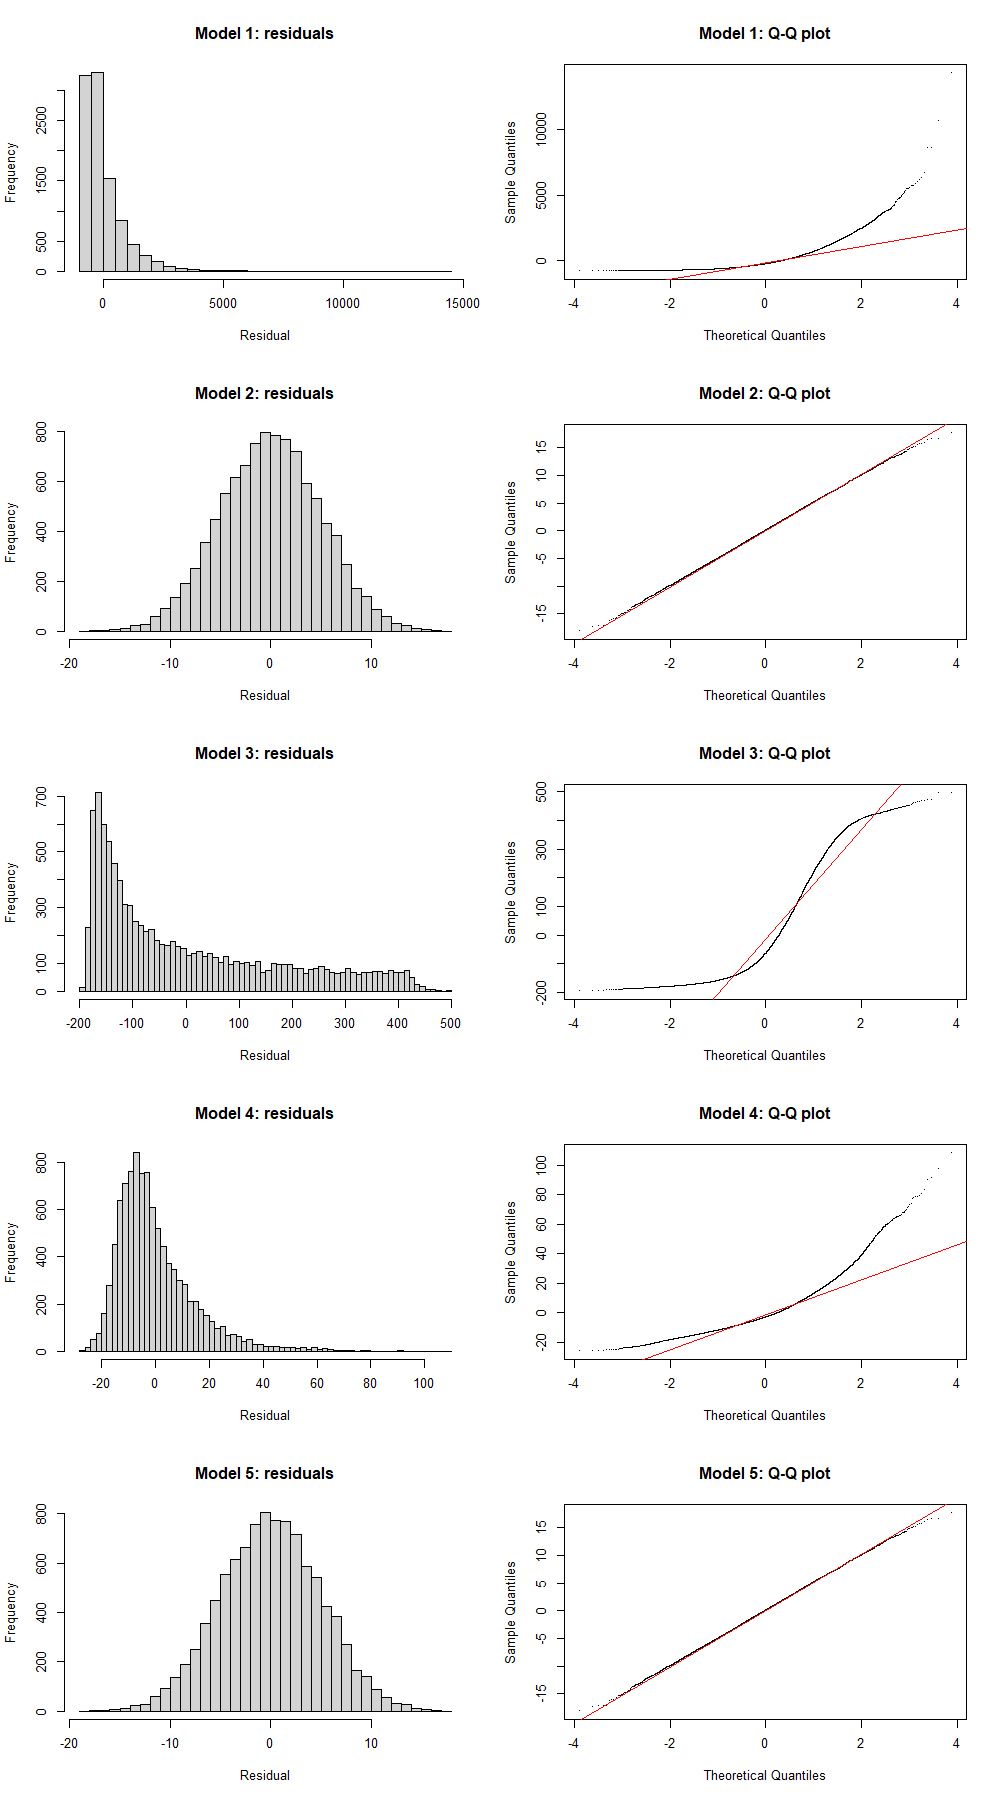
\includegraphics[width=0.72\textwidth]{fig5_residuals.png}
\caption{Residual histograms (left) and normal Q-Q plots (right) for the five candidate models.}
\label{fig:res}
\end{figure}

\subsection{Task 2.6: Selection of the best model}
Model~2 was chosen as the best model:
\begin{equation}
\hat{y}=4.4805\,x_4+1.2002\,x_1^3+0.8000\,x_3^4+120.02
\label{eq:best}
\end{equation}
The reasons are:
\begin{enumerate}
  \item \textbf{Information criteria:} it has the lowest AIC and the lowest BIC of the five models (\texttt{which.min()} returns 2 for both).
  \item \textbf{Residuals:} its residuals are symmetric, close to normal on the Q-Q plot, and pass the Shapiro--Wilk test. This is what we expect when the model structure is right and only the Gaussian measurement noise is left.
  \item \textbf{Parsimony:} Model~5 fits equally well but adds an $x_1^2$ term whose coefficient is almost zero ($-0.010$), so the term is not needed. According to \citet{burnham2002}, an AIC difference under 2 means that both models have support, so the decision rests on BIC, which favours Model~2 by 8.9 (strong evidence), and on choosing the simpler model. Model~2 is exactly Model~5 with $\theta_2=0$.
\end{enumerate}
The estimated coefficients are also very close to round numbers (0.8, 1.2, 4.48 and 120). This suggests that the simulated data were produced by a model with this exact structure, so Model~2 is very likely the ``true'' model.

\subsection{Task 2.7: Train/test validation and confidence intervals}
The data were split at random into 7000 training and 3000 test rows (\texttt{set.seed(123)}, Appendix~\ref{app:task2}, ``Task 2.7''). The same row indices were used for $\mathbf{X}$ and $\mathbf{y}$. Model~2 was refitted on the training rows only.

\textbf{1. Parameter estimates (training data).} $\hat\theta_1=4.4640$ ($x_4$), $\hat\theta_2=1.20015$ ($x_1^3$), $\hat\theta_3=0.800002$ ($x_3^4$) and $\hat\theta_{bias}=120.109$. These are almost identical to the full-data estimates, so the fit is stable.

\textbf{2. Test predictions.} On the 3000 unseen test rows the model reached an RMSE of 5.04\,W and $R^2=0.99996$. The RMSE is almost exactly the noise level estimated in Task~2.3 ($\hat\sigma\approx5.0$), so the model does not overfit: its test error is the noise floor. Figure~\ref{fig:predact} shows that all test predictions lie on the $y=x$ line.

\begin{figure}[H]
\centering
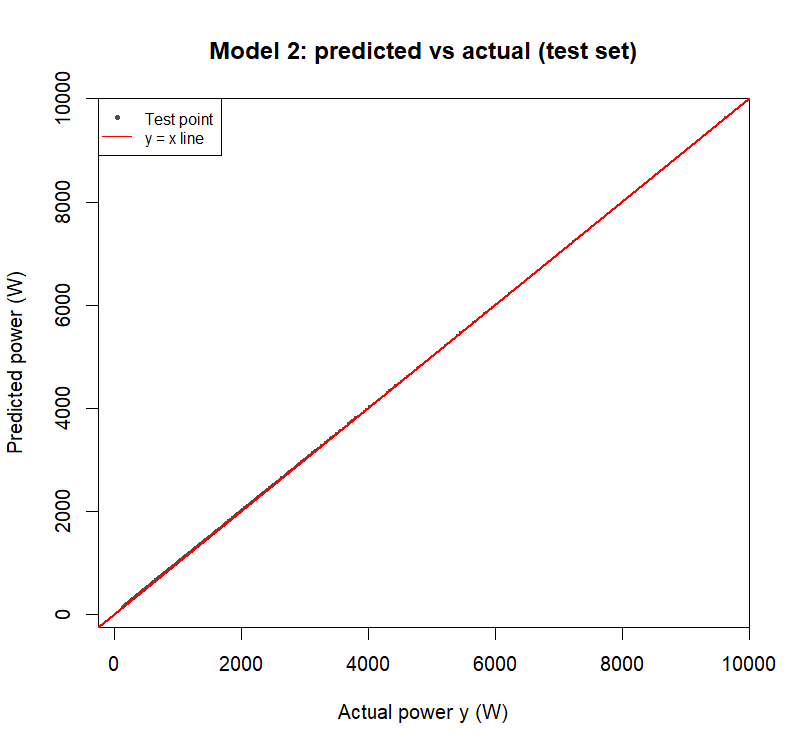
\includegraphics[width=0.55\textwidth]{fig6b_pred_vs_actual.png}
\caption{Predicted vs actual power for all 3000 test samples (Model~2 trained on 70\% of the data).}
\label{fig:predact}
\end{figure}

\textbf{3. 95\% confidence intervals.} The covariance of the estimates was computed as $\hat\sigma^2(\mathbf{X}_{tr}^T\mathbf{X}_{tr})^{-1}$ with $\hat\sigma^2=\text{RSS}_{tr}/(n_{tr}-k)$, and the critical value was $t_{0.975,6996}=1.960$. Figure~\ref{fig:ci} shows the first 40 test samples. In the top panel the predictions (red crosses) lie on top of the observed values (grey dots). The confidence intervals are very narrow, with a median width of only 0.38\,W (range 0.24--2.28\,W). On a scale of thousands of watts the error bars are shorter than the plotting symbols, so the bottom panel plots each point relative to its prediction, where the error bars (blue) can be seen.

\begin{figure}[H]
\centering
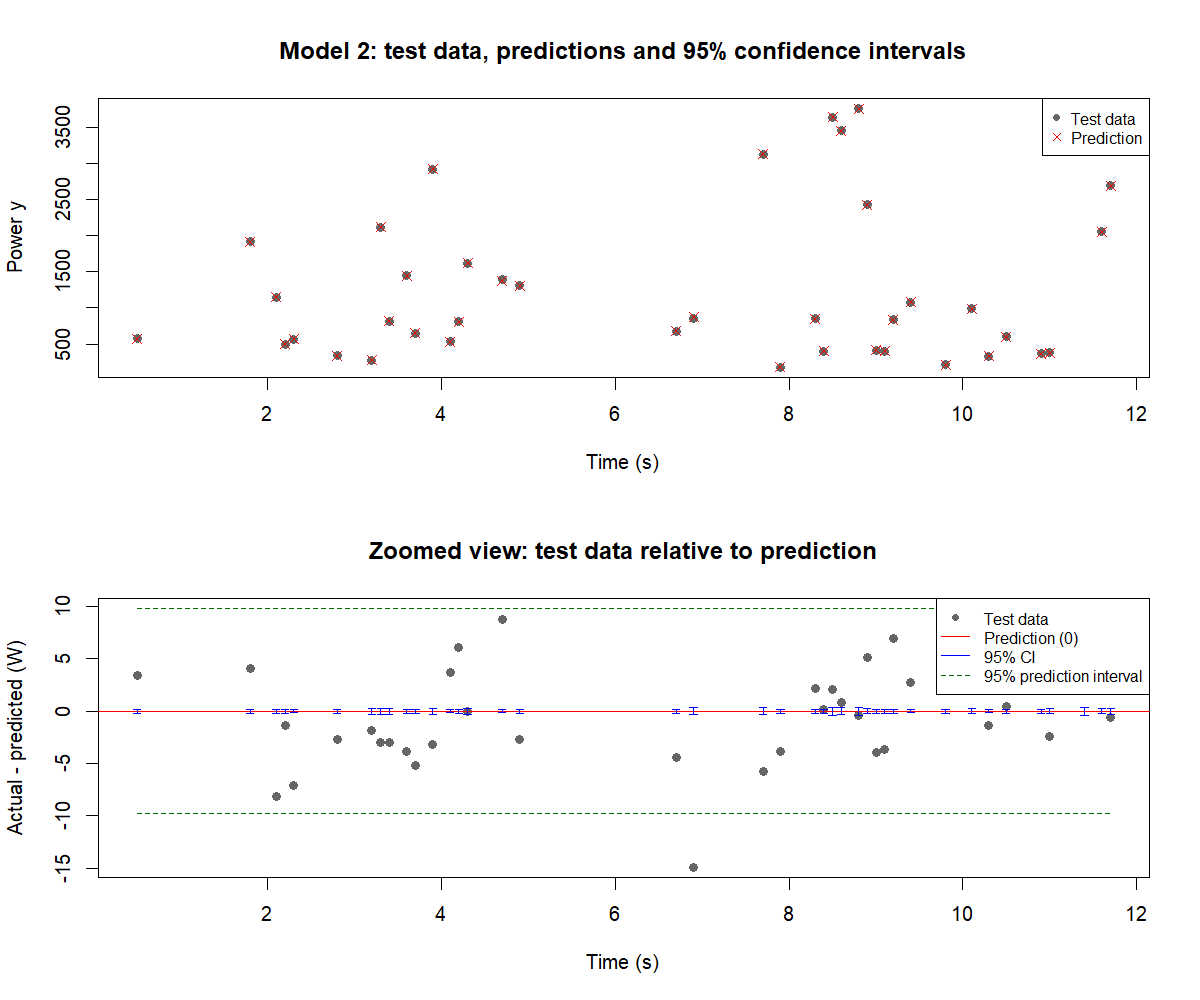
\includegraphics[width=0.95\textwidth]{fig6_confidence_intervals.png}
\caption{Model~2 predictions with 95\% confidence intervals for the first 40 test samples. Top: actual vs predicted power. Bottom: zoomed view of actual minus predicted, with 95\% confidence-interval error bars (blue) and 95\% prediction interval (dashed green).}
\label{fig:ci}
\end{figure}

It is important to tell the two kinds of interval apart. The confidence interval shows the uncertainty in the \emph{mean} prediction, which comes only from the uncertainty in $\hat{\boldsymbol\theta}$. With 7000 training samples this uncertainty is tiny, and only 3.7\% of the actual test values fall inside these intervals. That is expected, not a failure. The prediction interval adds the noise of a single new observation and is about $\pm9.8$\,W wide (total width 19.6\,W). It contains 94.6\% of the test values, very close to the nominal 95\%. This shows that the model and its error assumptions are well calibrated. The CI is widest for inputs far from the centre of the data, such as large $x_3$, because $x_3^4$ grows quickly there.

\section{Task 3: Approximate Bayesian Computation (ABC)}
\label{sec:task3}

Least squares gives one best value for each parameter. A Bayesian approach instead gives a full posterior distribution, which shows which values are plausible and how the parameters depend on each other. Rejection ABC approximates the posterior without writing down the likelihood: it only needs to simulate model output and compare it with the data \citep{beaumont2002,sunnaker2013}. The code is in Appendix~\ref{app:task3}.

\subsection{Task 3.1: Choice of parameters}
The Model~2 estimates were ranked by absolute value with R's \texttt{order()} function (Appendix~\ref{app:task3}, ``Task 3.1''). The two largest are $\theta_{bias}=120.022$ and $\theta_1=4.4805$ (the $x_4$ coefficient), so these two were estimated with ABC. The other two were fixed at their least squares values, $\theta_2=1.20018$ ($x_1^3$) and $\theta_3=0.800003$ ($x_3^4$).

\subsection{Task 3.2: Uniform priors}
A uniform prior was placed around each least squares estimate. To set a sensible width, the standard errors of the estimates were computed from $\hat\sigma^2(\mathbf{X}^T\mathbf{X})^{-1}$: $\text{SE}(\theta_{bias})=0.0978$ and $\text{SE}(\theta_1)=0.0167$. Each prior was set to the estimate $\pm10$ standard errors:
\begin{align*}
\theta_{bias}&\sim U(119.045,\;121.000),\\
\theta_1&\sim U(4.3135,\;4.6475).
\end{align*}
This range is wide enough to cover all plausible values, since the true value lies within a few standard errors of the estimate. It is also narrow enough that a useful share of the draws is accepted. A prior of $\pm50\%$ of the estimate would accept almost nothing, because these parameters are known so precisely.

\subsection{Task 3.3: Rejection ABC}
The algorithm used was:
\begin{enumerate}
  \item Draw $N=100{,}000$ pairs $(\theta_{bias}^{(j)},\theta_1^{(j)})$ independently from the two uniform priors, with the random seed fixed at 456 so that the run can be repeated.
  \item For each pair, compute the model output, with $\theta_2,\theta_3$ fixed:
  \[\hat{\mathbf y}^{(j)}=\theta_{bias}^{(j)}+\theta_1^{(j)}x_4+\theta_2x_1^3+\theta_3x_3^4.\]
  \item Measure the distance from the data as $\text{RSS}^{(j)}=\sum_i(y_i-\hat y_i^{(j)})^2$.
  \item Accept the pair if $\text{RSS}^{(j)}\le\epsilon$, with $\epsilon=1.0005\times\text{RSS}_{LS}=250935.9$, that is, if it fits within 0.05\% of the best possible fit.
\end{enumerate}
The tolerance allows the RSS to rise by 125.4, which is about $5\hat\sigma^2$, or a drop of about 2.5 in the log-likelihood. A tolerance on this scale keeps parameter values that are statistically compatible with the data. The RSS of the prior draws ranged from 250{,}811 to 275{,}113. In total, \textbf{1921 draws were accepted} (an acceptance rate of 1.92\%), enough for stable histograms.

\subsection{Task 3.4: Joint and marginal posterior distributions}
Figure~\ref{fig:abc} shows the accepted samples. The left panel is the joint posterior and the other two panels are the marginal posteriors. The red markers show the least squares estimates. Table~\ref{tab:abc} summarises the posteriors.

\begin{figure}[H]
\centering
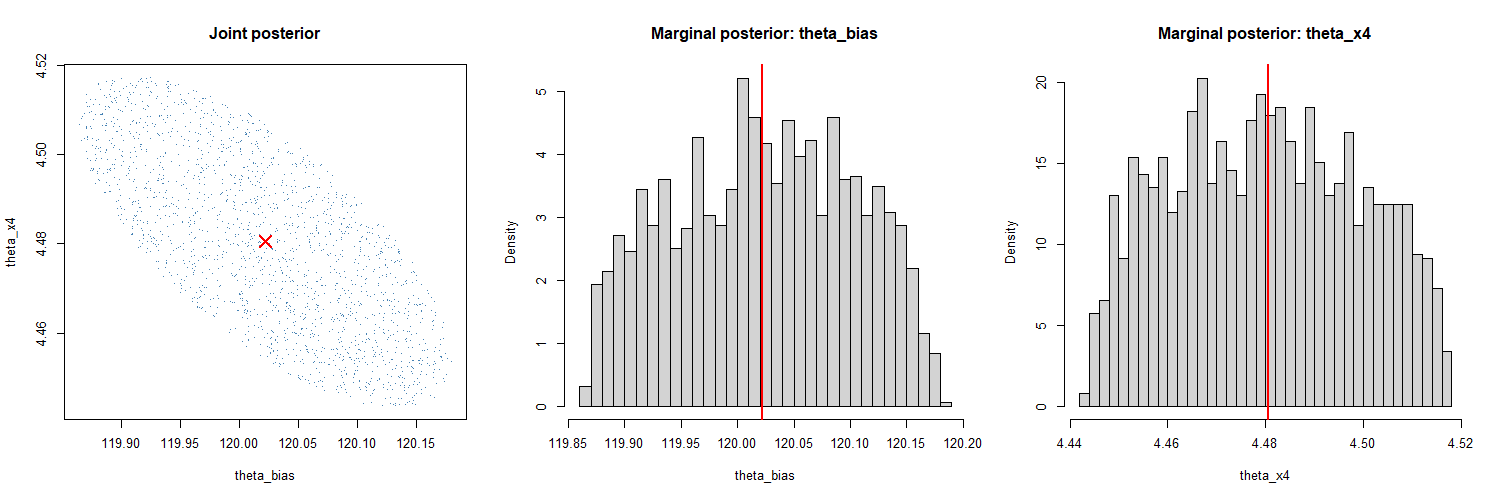
\includegraphics[width=\textwidth]{fig7_abc_posterior.png}
\caption{Rejection ABC results for Model~2: joint posterior of $(\theta_{bias},\theta_{x_4})$ (left) and marginal posteriors (centre, right). The red markers show the least squares estimates.}
\label{fig:abc}
\end{figure}

\begin{table}[H]
\centering
\caption{Posterior summaries from 1921 accepted ABC samples.}
\label{tab:abc}
\small
\begin{tabular}{lccccc}
\toprule
Parameter & LS est. & Post.\ mean & Post.\ SD & 95\% cred.\ interval & Prior range \\
\midrule
$\theta_{bias}$ & 120.022 & 120.023 & 0.079 & [119.881, 120.157] & [119.045, 121.000] \\
$\theta_1$ ($x_4$) & 4.4805 & 4.4799 & 0.019 & [4.4479, 4.5134] & [4.3135, 4.6475] \\
\bottomrule
\end{tabular}
\end{table}

\subsection{Task 3.5: Explanation of the results}
\textbf{Agreement with least squares.} Both posterior means agree with the least squares estimates to three or four significant figures, and both estimates lie in the centre of the joint cloud. This is expected: with a flat prior, the posterior is driven by the likelihood, and least squares is the maximum likelihood estimate.

\textbf{Learning from the data.} The posterior ranges are much narrower than the priors. The 95\% credible interval of $\theta_{bias}$ (width 0.28) covers only about 14\% of the prior width of 1.96, and that of $\theta_1$ (width 0.066) about 20\% of the prior width of 0.33. The data have greatly reduced the uncertainty. Both intervals exclude zero by a wide margin, so network traffic has a clear positive effect on power ($\approx4.5$\,W per unit of $x_4$), even though Task~1 showed almost no correlation between $x_4$ and $y$ on its own. The idle power is about 120\,W.

\textbf{Correlation between parameters.} The joint posterior is a tilted ellipse with correlation $-0.71$. Network traffic is always positive (mean 3.0), so a larger $\theta_1$ raises every prediction by about $3\,\Delta\theta_1$. A smaller intercept can cancel this. The data cannot fully separate the two effects, so they trade off against each other. This information is lost if the parameters are reported one at a time.

\textbf{Shape of the posterior.} The marginal histograms are rounded and fairly flat on top rather than bell-shaped. This comes from the method. A fixed RSS threshold accepts every draw inside an ellipse of nearly equal fit, and because the prior is uniform, the accepted points are spread almost evenly inside that ellipse. A smaller tolerance (with more draws), or a version that adds simulated Gaussian noise to each output, would give a shape closer to the true Gaussian posterior. The location, spread and correlation would stay much the same.

\section{Discussion}
\label{sec:discussion}

\textbf{What the model says about the server.} The selected model (Equation~\ref{eq:best}) splits power into four parts:
\begin{itemize}
  \item a fixed idle power of about 120\,W, drawn even when the load is zero, which matches the observation that servers are not energy proportional \citep{barroso2007};
  \item a cubic CPU term ($1.2\,x_1^3$), which fits the common view that dynamic CPU power rises faster than linearly as clock speed and voltage increase together;
  \item a fourth-power disk I/O term ($0.8\,x_3^4$), which is by far the largest source of variation and causes the rare, very high power peaks;
  \item a small linear network term ($4.48\,x_4$).
\end{itemize}
Memory usage ($x_2$) does not appear in the selected model. Model~4, which uses $x_2$ in place of $x_4$, was much worse ($\Delta\text{BIC}>21{,}000$), and $x_2$ was not significant in the baseline linear model. Because the data are simulated, these terms describe how the data were generated and should not be read as a physical law. The pattern is still realistic: storage-heavy and compute-heavy workloads drive power far more than memory use does.

\textbf{Agreement between methods.} Several independent pieces of evidence point to Model~2: the large drop in RSS, the lowest AIC and BIC, Gaussian residuals, a test RMSE equal to the noise level, a 95\% prediction interval with 94.6\% coverage, and ABC posteriors centred on the least squares values. Each check tests a different property, such as in-sample fit, model complexity, error structure, out-of-sample accuracy, interval calibration and parameter uncertainty. Their agreement gives strong confidence in the choice.

\textbf{Exploratory analysis can mislead.} Task~1 alone would have suggested that network traffic does not matter, since $r=0.010$. Yet the regression shows a clear effect with a very small standard error (0.017), and leaving out $x_4$ (as Model~4 does) raises the RSS by a factor of eight. A small effect can be hidden in pairwise plots by the much larger variation from another input. Variables should therefore not be dropped on the basis of correlations alone.

\textbf{Choosing between nested models.} Model~5 contains Model~2, so its RSS is always at least as low. Choosing a model by RSS or $R^2$ alone would pick the larger model every time. AIC and BIC penalise the extra parameter. In this case $\Delta\text{AIC}=1.67$ is borderline, while $\Delta\text{BIC}=8.9$ is decisive. With large samples BIC is consistent: it tends to pick the true model when that model is among the candidates \citep{schwarz1978,burnham2002}. This matches what we see here.

\textbf{Limitations.}
\begin{itemize}
  \item The brief states that the \emph{inputs} also contain noise. Least squares assumes the inputs are measured exactly. Noise in the inputs biases the estimates towards zero, and the bias grows when inputs are raised to high powers. The coefficients here are so close to round numbers that the input noise seems to be small, but in real telemetry this could matter.
  \item The variance in Task~2.3 uses $n-1$, as the brief requires, rather than the unbiased $n-k$. With $n=10{,}000$ the difference is negligible and does not change the ranking.
  \item The Shapiro--Wilk test was run on a random sample of 5000 residuals. With very large samples, formal tests can reject normality for tiny departures, so the Q-Q plots are the main evidence.
  \item The ABC distance is computed from the deterministic model output, without simulated noise, and with a fixed RSS tolerance. As explained in Section~\ref{sec:task3}, this shapes the posterior. Only two of the four parameters were treated as uncertain, so the posterior is conditional on the other two being fixed, and it understates the full uncertainty.
  \item Only the five given models were compared. A model outside this set, for example one with interaction terms, could not be found by this procedure.
\end{itemize}

\textbf{Reflection.} Writing the least squares solution by hand instead of only calling \texttt{lm()} made each step clear, and checking against \texttt{lm()} gave confidence that the code was correct. The most useful lesson was to look at residual plots and test-set behaviour as well as the numbers. For example, the 3.7\% coverage of the confidence interval looked like an error at first, but it is the correct result once the confidence interval is separated from the prediction interval.

\section{Conclusion}
\label{sec:conclusion}

This report modelled simulated cloud server power consumption from four telemetry inputs using polynomial regression. The exploratory analysis showed stationary, independent samples. Disk I/O was strongly and non-linearly linked to power, CPU weakly, and memory and network showed no visible link. A linear model explained only 76\% of the variance and left clearly non-Gaussian residuals.

Of the five candidate models, \textbf{Model~2}, $y=4.48\,x_4+1.20\,x_1^3+0.80\,x_3^4+120.0$, was selected. It had the lowest AIC (60607.9) and BIC (60636.7), and its residuals were the only ones, together with those of the over-parameterised Model~5, that were consistent with Gaussian noise of standard deviation about 5\,W. When trained on 70\% of the data, it predicted the remaining 30\% with an RMSE of 5.04\,W and $R^2=0.99996$, and its 95\% prediction intervals covered 94.6\% of the test values.

Rejection ABC on the two largest parameters gave posterior means of 120.02 for the intercept and 4.480 for the network coefficient, with narrow 95\% credible intervals and a negative correlation of $-0.71$ between them. These results confirm the least squares estimates and add information about how the two parameters depend on each other.

In practice, a model of this kind could estimate server power from software telemetry alone, without hardware meters, and help with energy-aware scheduling. Future work could use errors-in-variables regression to handle noise in the inputs, ABC on all four parameters with a smaller tolerance, and testing on real server measurements.


% ---- References ----
\newpage
% Reference list in Harvard (author-year) style.
% Written out by hand so the project compiles without a BibTeX/Biber run
% (keeps compile time inside the Overleaf free-plan limit).
\begin{thebibliography}{99}
\addcontentsline{toc}{section}{References}

\bibitem[Akaike(1974)]{akaike1974}
Akaike, H. (1974) `A new look at the statistical model identification', \emph{IEEE Transactions on Automatic Control}, 19(6), pp. 716--723.

\bibitem[Barroso and H{\"o}lzle(2007)]{barroso2007}
Barroso, L.A. and H{\"o}lzle, U. (2007) `The case for energy-proportional computing', \emph{Computer}, 40(12), pp. 33--37.

\bibitem[Beaumont et~al.(2002)]{beaumont2002}
Beaumont, M.A., Zhang, W. and Balding, D.J. (2002) `Approximate Bayesian computation in population genetics', \emph{Genetics}, 162(4), pp. 2025--2035.

\bibitem[Burnham and Anderson(2002)]{burnham2002}
Burnham, K.P. and Anderson, D.R. (2002) \emph{Model Selection and Multimodel Inference: A Practical Information-Theoretic Approach}. 2nd edn. New York: Springer.

\bibitem[Fan et~al.(2007)]{fan2007}
Fan, X., Weber, W.-D. and Barroso, L.A. (2007) `Power provisioning for a warehouse-sized computer', in \emph{Proceedings of the 34th Annual International Symposium on Computer Architecture (ISCA '07)}, pp. 13--23.

\bibitem[James et~al.(2013)]{james2013}
James, G., Witten, D., Hastie, T. and Tibshirani, R. (2013) \emph{An Introduction to Statistical Learning: with Applications in R}. New York: Springer.

\bibitem[Montgomery et~al.(2012)]{montgomery2012}
Montgomery, D.C., Peck, E.A. and Vining, G.G. (2012) \emph{Introduction to Linear Regression Analysis}. 5th edn. Hoboken, NJ: Wiley.

\bibitem[Pritchard et~al.(1999)]{pritchard1999}
Pritchard, J.K., Seielstad, M.T., Perez-Lezaun, A. and Feldman, M.W. (1999) `Population growth of human Y chromosomes: a study of Y chromosome microsatellites', \emph{Molecular Biology and Evolution}, 16(12), pp. 1791--1798.

\bibitem[{R Core Team}(2026)]{rcore2026}
R Core Team (2026) \emph{R: A Language and Environment for Statistical Computing}. Version 4.6.1. Vienna, Austria: R Foundation for Statistical Computing.

\bibitem[Schwarz(1978)]{schwarz1978}
Schwarz, G. (1978) `Estimating the dimension of a model', \emph{The Annals of Statistics}, 6(2), pp. 461--464.

\bibitem[Shapiro and Wilk(1965)]{shapiro1965}
Shapiro, S.S. and Wilk, M.B. (1965) `An analysis of variance test for normality (complete samples)', \emph{Biometrika}, 52(3--4), pp. 591--611.

\bibitem[Sunn{\aa}ker et~al.(2013)]{sunnaker2013}
Sunn{\aa}ker, M., Busetto, A.G., Numminen, E., Corander, J., Foll, M. and Dessimoz, C. (2013) `Approximate Bayesian computation', \emph{PLoS Computational Biology}, 9(1), e1002803.

\end{thebibliography}


% ---- Appendix ----
\newpage
\appendix
\section{R Code}
\label{app:code}

All code is written in base R (version 4.6.1) and is split into three scripts, one for each task. Each script is run from the project folder that contains \texttt{data/}, \texttt{scripts/} and \texttt{figures/}. The Task~3 script reuses the objects created in Task~2 and runs the Task~2 script itself if they do not exist yet. Comments in the code mark each sub-task (Task 1.1, Task 2.3, and so on), and these match the section headings in the report.

\subsection{Task 1: Preliminary data analysis}
\label{app:task1}
\lstinputlisting[caption={Task 1 -- \texttt{task1\_data\_exploration.R}}]{scripts/task1_data_exploration.R}

\subsection{Task 2: Regression (Tasks 2.1--2.7)}
\label{app:task2}
\lstinputlisting[caption={Task 2 -- \texttt{task2\_regression.R}}]{scripts/task2_regression.R}

\subsection{Task 3: Approximate Bayesian Computation}
\label{app:task3}
\lstinputlisting[caption={Task 3 -- \texttt{task3\_abc.R}}]{scripts/task3_abc.R}


\end{document}
